%%%%%%%%%%%%%%%%%%%%%%%%%%%%%%%%%%%%%%%%%%%%%%%%%%%%%%%%%%%%%%%%%%%%%%%%%%%%%%%%
%%%% Glyphs I need commands for %%%%%%%%%%%%%%%%%%%%%%%%%%%%%%%%%%%%%%%%%%%%%%%%
% Glyph addresses taken from:
% http://www.macosxhints.com/article.php?story=20071028203517911
% OS X 10.6 uses Lucida Grande for these symbols
\newcommand{\shiftkey}      {\textsf{⇧}} % U+21E7
\newcommand{\controlkey}    {\textsf{⌃}} % U+2303
\newcommand{\optionkey}     {\textsf{⌥}} % U+2325
\newcommand{\commandkey}    {\textsf{⌘}} % U+2318
\newcommand{\deleterightkey}{\textsf{⌦}} % U+2326
\newcommand{\deleteleftkey} {\textsf{⌫}} % U+232B
\newcommand{\escapekey}     {\textsf{⎋}} % U+238B
\newcommand{\returnkey}     {\textsf{↩}} % U+21A9
\newcommand{\leftkey}       {\textsf{←}} % U+2190
\newcommand{\upkey}         {\textsf{↑}} % U+2191
\newcommand{\rightkey}      {\textsf{→}} % U+2192
\newcommand{\downkey}       {\textsf{↓}} % U+2193
\newcommand{\tabkey}        {\textsf{⇥}} % U+21E5


%%%%%%%%%%%%%%%%%%%%%%%%%%%%%%%%%%%%%%%%%%%%%%%%%%%%%%%%%%%%%%%%%%%%%%%%%%%%%%%% 
%%%%%%%%%%%%%%%%%%%%%%%%%%%%%%%%%%%%%%%%%%%%%%%%%%%%%%%%%%%%%%%%%%%%%%%%%%%%%%%% 

\renewcommand*{\descriptionlabel}[1]{\hspace\labelsep\normalfont #1}
\newcommand{\keys}[1]{\textsf{#1}}
\newcommand{\command}[1]{\texttt{\textbf{#1}}}
\newcommand{\namedfield}[1]{{\normalfont\emph{〈#1〉}}} % 〈#1〉
\newcommand{\menu}[1]{\textsf{#1}}
\newcommand{\menusep}{\ensuremath{\mathsf{\to}} }
\newcommand{\noun}[1]{\textsf{#1}}
\newcommand{\make}[1]{\textit{#1}}
\newcommand{\model}[1]{\texttt{#1}}
\newcommand{\makemodel}[2]{\make{#1} \model{#2}}

%%%%%%%%%%%%%%%%%%%%%%%%%%%%%%%%%%%%%%%%%%%%%%%%%%%%%%%%%%%%%%%%%%%%%%%%%%%%%%%%
%%%% Labelled style %%%%%%%%%%%%%%%%%%%%%%%%%%%%%%%%%%%%%%%%%%%%%%%%%%%%%%%%%%%%
\newcommand*{\pxilabelled}[1]{\hspace\labelsep \normalfont\bfseries #1}

%%%%%%%%%%%%%%%%%%%%%%%%%%%%%%%%%%%%%%%%%%%%%%%%%%%%%%%%%%%%%%%%%%%%%%%%%%%%%%%%
%%%% Common expressions %%%%%%%%%%%%%%%%%%%%%%%%%%%%%%%%%%%%%%%%%%%%%%%%%%%%%%%%
\newcommand{\seeref}[1]{see \ref{#1}, p.{} \pageref{#1}}
\newcommand{\secnameref}[1]{\S\ref{#1}~\nameref{#1}}

%%%%%%%%%%%%%%%%%%%%%%%%%%%%%%%%%%%%%%%%%%%%%%%%%%%%%%%%%%%%%%%%%%%%%%%%%%%%%%%%
%%%% New Environments %%%%%%%%%%%%%%%%%%%%%%%%%%%%%%%%%%%%%%%%%%%%%%%%%%%%%%%%%%

%%%% Lengths for boxes %%%%%%%%%%%%%%%%%
\newlength{\mysymbolheight}
\setlength{\mysymbolheight}{2em}

%%%% Symbols for boxes %%%%%%%%%%%%%%%%%
\newcommand{\warningsign}{\dejavusans{}⚠\normalfont}
\newcommand{\checkmark}{\dejavusans{}✗\normalfont}
\newcommand{\ballotx}{\dejavusans{}✓\normalfont}

%%%%%%%%%%%%%%%%%%%%%%%%%%%%%%%%%%%%%%%% Please Avoid %%%%%%%%%%%%%%%%%%%%%%%%%%
\newenvironment{avoid}%
{\begin{list}{}%
    {\setlength{\leftmargin}{\mysymbolheight}}%
    {\setlength{\parindent}{-2cm}}%
    \item[]%
      {\fontsize{\mysymbolheight}{1em}\hspace{-\mysymbolheight}\warningsign} \textbf{\sffamily AVOID}}
{\end{list}}

%%%%%%%%%%%%%%%%%%%%%%%%%%%%%%%%%%%%%%%% Please DO NOT %%%%%%%%%%%%%%%%%%%%%%%%%
\newenvironment{pleasedonot}%
{\begin{list}{}%
    {\setlength{\leftmargin}{\mysymbolheight}}%
    {\setlength{\parindent}{-2cm}}%
    \item[]%
      {\fontsize{\mysymbolheight}{1em}\hspace{-\mysymbolheight}\checkmark} \textbf{\sffamily DO NOT}}
{\end{list}}

%%%%%%%%%%%%%%%%%%%%%%%%%%%%%%%%%%%%%%%% Please DO  %%%%%%%%%%%%%%%%%%%%%%%%%%%%
\newenvironment{pleasedo}%
{\begin{list}{}%
    {\setlength{\leftmargin}{\mysymbolheight}}%
    {\setlength{\parindent}{-2cm}}%
    \item[]%
      {\fontsize{\mysymbolheight}{1em}\hspace{-\mysymbolheight}\ballotx} \textbf{\sffamily DO}}
{\end{list}}

\newenvironment{note}%
{\noindent\par \itshape \small Note:\:}
{}




%%%%%%%%%%%%%%%%%%%%%%%%%%%%%%%%%%%%%%%%%%%%%%%%%%%%%%%%%%%%%%%%%%%%%%%%%%%%%%%%
%%%% Title Page %%%%%%%%%%%%%%%%%%%%%%%%%%%%%%%%%%%%%%%%%%%%%%%%%%%%%%%%%%%%%%%%
\renewcommand*{\maketitle}{
  \begin{figure}[p]\centering
  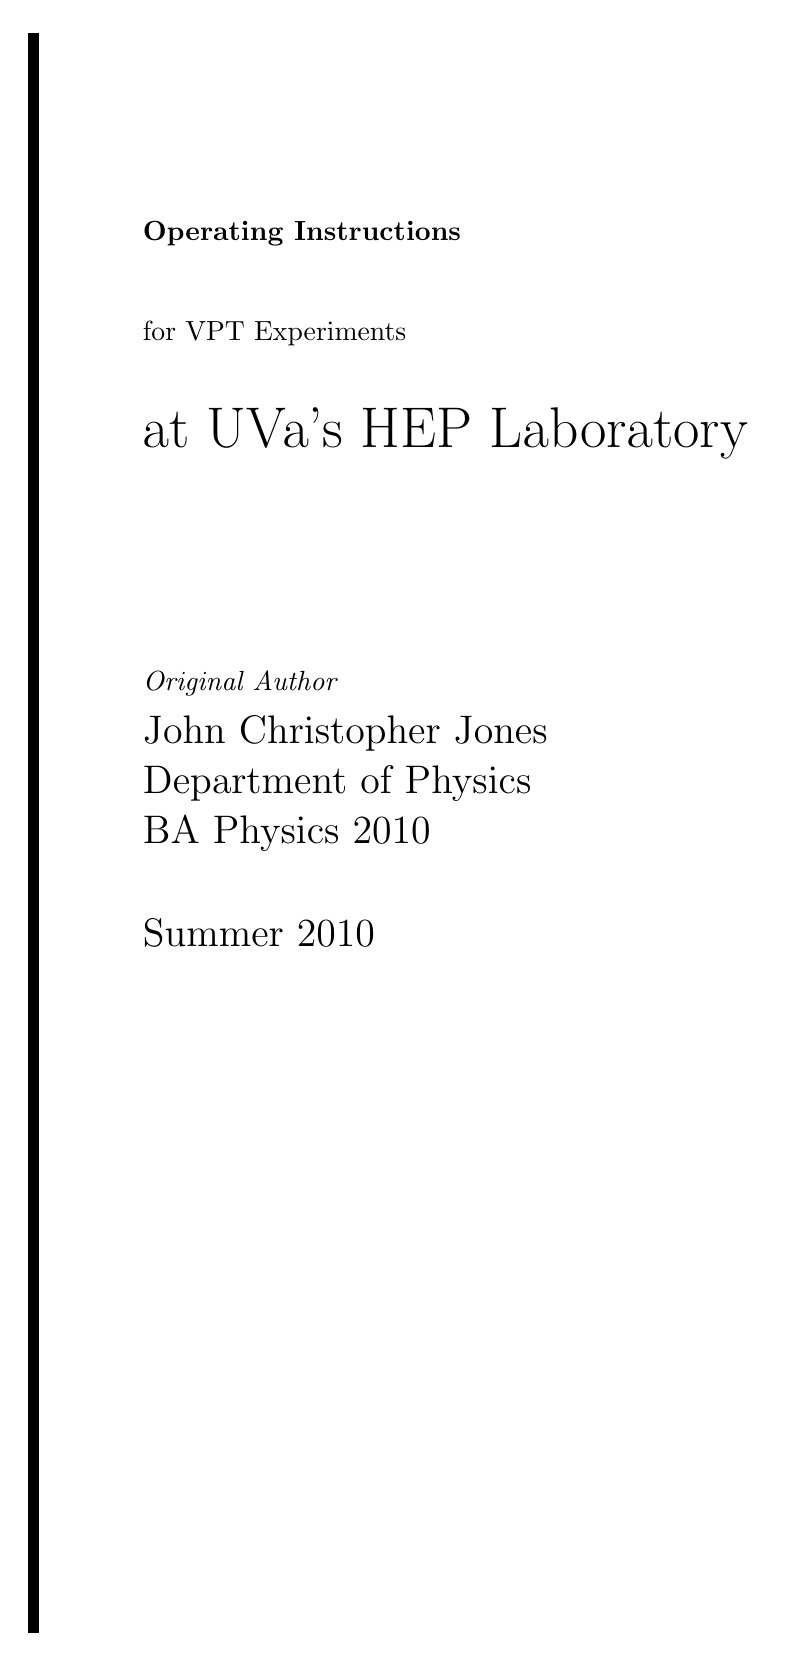
\begin{tikzpicture}
    \draw[line width=4pt] (2in,0in) -- ++(down:8in);
    \begin{scope}[yshift=-1in,xshift=-.5in]
      \draw (3in,0)      node[anchor=west] {\HUGE \bfseries Operating Instructions};
      \draw (3in,-.5in)  node[anchor=west] {\HUGE for VPT Experiments};
      \draw (3in,-1in)   node[anchor=west] {\huge at UVa's HEP Laboratory};
      \draw (3in,-2.25in)   node[anchor=west] {\itshape Original Author};
      \draw (3in,-2.5in) node[anchor=west] {\Large John Christopher Jones};
      \draw (3in,-2.75in) node[anchor=west] {\Large Department of Physics};
      \draw (3in,-3.0in) node[anchor=west] {\Large BA Physics 2010};
      \draw (3in,-3.5in) node[anchor=west] {\Large Summer 2010};
      % \draw (3in,  -5in) node[anchor=west,red] {\HUGE \bfseries [DRAFT]};
    \end{scope}
  \end{tikzpicture}
  \end{figure}
\newpage}

%%% Local Variables: 
%%% mode: latex
%%% TeX-master: "Manual"
%%% End: 
